\documentclass[11pt,letterpaper]{article}
\usepackage[margin=1.0in]{geometry}
\usepackage[utf8]{inputenc}
\usepackage{cite}
\usepackage{amsmath}
\usepackage{amsfonts}
\usepackage{amssymb}
\usepackage{makeidx}
\usepackage{graphicx}
\usepackage{hyperref}
\setlength\parindent{0pt}

\author{STUDENT NAME}
\title{Lab4: Frequency domain analysis of First Order Systems (Passive Filters)}

\begin{document}

\maketitle

\section{Objectives}

The objective of this lab is to understand the functioning of two RC networks being a low pass and a high pass filter in the Frequency domain.

\section{Introduction}

Filters are used to suppress undesired frequencies in signals (such as noise) and to avoid a phenomenon called aliasing. RC passive filters are simple in design, but have limited performance. In this lab you will analyze the frequency domain behavior of these filters using an oscilloscope.

\subsection{Low pass filter:}

A low pass filter passes low frequencies and rejects high frequencies from the input signal. A first order, low pass RC filter is an RC series circuit across the input, with the output taken across the capacitor. We assume that the output of the circuit is connected only to high impedance (not connected), so that the current is the same in both R and C. 

\begin{figure}
\centering
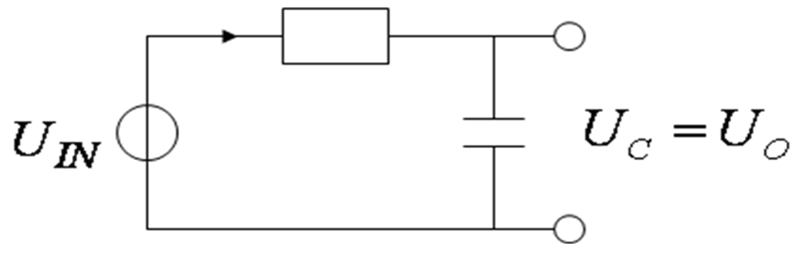
\includegraphics[width=0.7\linewidth]{Lab4_LowPassFilter}
\caption{An RC network configured as a Low Pass Filter.}
\label{fig:Lab4_LowPassFilter}
\end{figure}

The transfer function of the low-pass filter can be written as follows by simply substituting $s = j \omega$  from the Laplace domain description:

\begin{equation} \label{Eqn:PassiveFilters1}
G(j \omega) = \dfrac{U_O (j \omega)}{U_{IN} (j \omega)} = \dfrac{1}{1 + j \omega \tau}
\end{equation}

\subsection{High pass filter:}

\begin{figure}
\centering
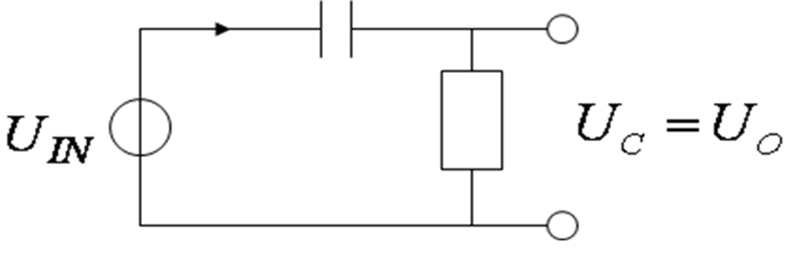
\includegraphics[width=0.7\linewidth]{Lab4_HighPassFilter}
\caption{An RC network configured as a High Pass Filter.}
\label{fig:Lab4_HighPassFilter}
\end{figure}

A high pass filter passes high frequencies and rejects low frequencies. The transfer function of the high-pass filter can be written as follows:

\begin{equation} \label{Eqn:PassiveFilters2}
G(j \omega) = \dfrac{U_O (j \omega)}{U_{IN} (j \omega)} = \dfrac{j \omega \tau}{1 + j \omega \tau}
\end{equation}
	
\section{Equipment}
	
\begin{enumerate}
\item Power supply
\item Bread board
\item Capacitor, 1 $nF$
\item Resistor, 100k
\item Function generator
\item Oscilloscope
\item DMM
\end{enumerate}
	 	
\section{Procedures}	 

\subsection{Simulation}

\begin{enumerate}
\item Use MatLab to simulate the behavior of a low-pass filter as shown in \ref{fig:Lab4_LowPassFilter}. Eqn \ref{Eqn:PassiveFilters1} shows the transfer function in the frequency domain. Choose $R = 100k, C = 1 nF$. Use the MatLab function \textbf{bode} to generate the Bode plot.
\item Repeat step 1 for the high pass filter. 
\end{enumerate}

\subsection{Measurement low pass filter}

\begin{enumerate}
\item Construct the simple schematic given in Fig 1 using a resistor of 100k (tolerance 5\%) and a capacitor of 1 $nF$.
\item Measure the "exact" value of the resistor using a multimeter.
\item Measure the "exact" value of the capacitor using a capacitance meter.
\item Compute the value of the time constant $\tau = RC$
\item Compute the value of the corner frequency $\omega _c$ in rad/s.
\item Convert the value from (5) to find the corner frequency $f_c$ in Hz.
\item Connect the power supply and put 5 Volt on the input of the circuit. Measure the DC output voltage using a voltmeter. Is this what you expected? 
\item Put a sine wave on the circuit. Find the -3dB point by measuring the input and output AC voltages with the DMM. Measure this by measuring the DC input component using the DMM (put it in DC mode). Show both input and output on the scope. You should have an approximate phase shift of 45 degrees. The ratio of the amplitudes should be $\dfrac{1}{\sqrt{2}}$  (-3dB point)
\end{enumerate}

Fill out the following table:\\

\begin{tabular}{|c|c|c|c|c|}
\hline  & Input voltage (AC) & Output voltage (AC) & Ratio Output/Input (dB) & Phase (deg) \\ 
\hline $f_c / 10$ &  &  &  &  \\ 
\hline $f_c $ &  &  &  &  \\ 
\hline $f_c * 10$ &  &  &  &  \\ 
\hline 
\end{tabular}\\ 

Show a Lissajous figure on the scope and try to compute the phase angle from it.

\subsection{Measurement high pass filter}

Reverse the capacitor and the resistor and repeat all steps from the low-pass filter section. Fill out the following table:\\

\begin{tabular}{|c|c|c|c|c|}
\hline  & Input voltage (AC) & Output voltage (AC) & Ratio Output/Input (dB) & Phase (deg) \\ 
\hline $f_c / 10$ &  &  &  &  \\ 
\hline $f_c $ &  &  &  &  \\ 
\hline $f_c * 10$ &  &  &  &  \\ 
\hline 
\end{tabular}\\

Figure \ref{fig:Lab4_LissajousFigures} shows the Lissajous figures for varying phase shifts. The phase shifts between input and output are from (a) to (f), 0, 45, 90, 135, 180, 315 degrees. The formula used to determine the phase shift is:

\begin{equation} \label{Eqn:PassiveFilters3}
\sin \theta = \dfrac{Y}{H}
\end{equation}
 
\begin{figure}
\centering
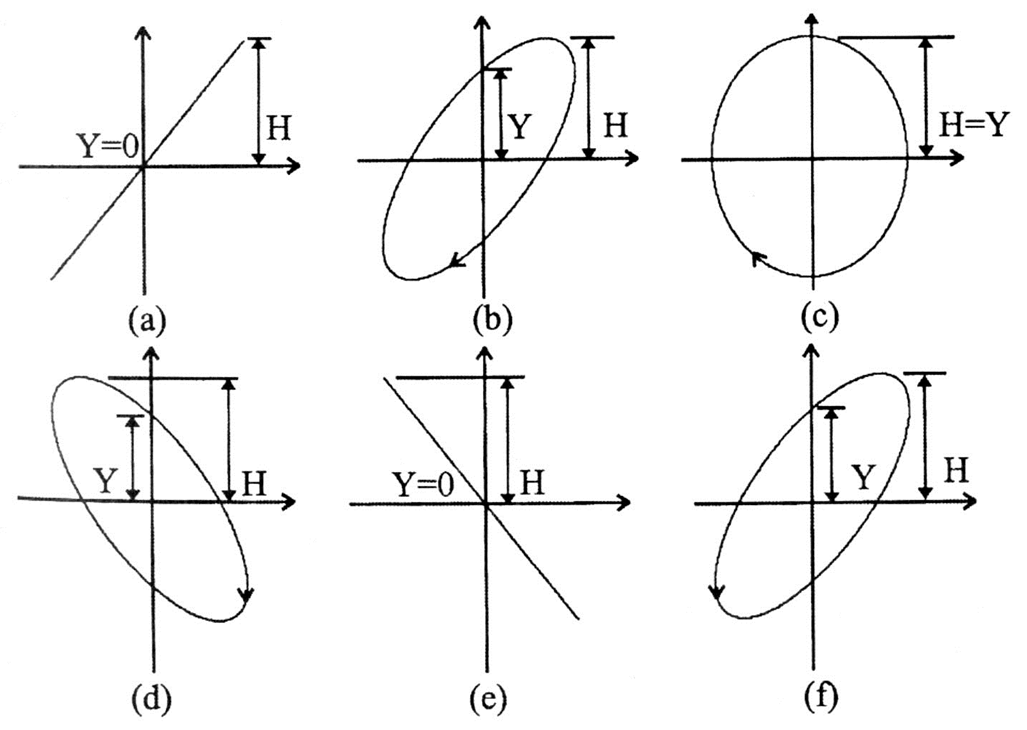
\includegraphics[width=0.7\linewidth]{Lab4_LissajousFigures}
\caption{Lissajous figures to study phase shift in filters.}
\label{fig:Lab4_LissajousFigures}
\end{figure}
 
\section{Questions}

Q1: Derive Eqn \ref{Eqn:PassiveFilters1} using the Impedance values of the resistor and capacitor and apply the voltage divider principle. Do this on paper, and then put in all equations here using the LaTex functionality.\\
A1:\\


Q2:	Explain why at the corner frequency for the low pass filter the amplitude drops by -3dB and you will have a phase shift of 45 degrees.\\
A2:\\

\end{document}
